\documentclass{standalone}
\usepackage{tikz}

\usetikzlibrary{arrows,calc,shapes,decorations.pathreplacing}

\begin{document}
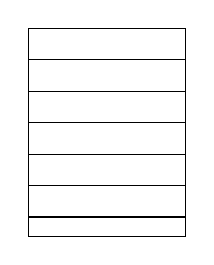
\begin{tikzpicture}
	\begin{scope}[every node/.style={draw, anchor=text, rectangle split,
		rectangle split parts=7,minimum width=2cm}]
    
	\node (cache) at (0,0){
		\nodepart{two}
		\nodepart{three}
		\nodepart{four} 
		\nodepart{five}
		\nodepart{six}
		\nodepart{seven} {
			
		}
	};
  \end{scope}
  
\end{tikzpicture}
\end{document}